\documentclass[12pt,a4paper]{report}
\usepackage[utf8]{inputenc}
\usepackage[T1]{fontenc}
\usepackage[french]{babel}
\usepackage{geometry}
\usepackage{graphicx}
\usepackage{longtable}
\usepackage{array}
\usepackage{fancyhdr}
\usepackage{hyperref}
\usepackage{amsmath}
\usepackage{titlesec}
\usepackage{float}
\usepackage{amssymb}
\usepackage{xcolor} % important pour utiliser \textcolor

\geometry{margin=2.5cm}
\pagestyle{fancy}
\fancyhf{}

\begin{document}

\thispagestyle{empty} % pas de numéro de page

\centering

% En-tête
{\large \textbf{République Tunisienne}}\\[0.2cm]
{\large \textbf{Ministère de l’Enseignement Supérieur et de la Recherche Scientifique}}\\[0.2cm]
{\large \textbf{Université de Monastir}}\\[0.2cm]
{\large \textbf{Institut Supérieur d’Informatique de Mahdia}}\\[0.8cm]

% Logo

\includegraphics[width=3.5cm]{isima.jpeg}\\[0.8cm]

% Ligne violette
\textcolor{violet}{\rule{\linewidth}{1pt}}\\[0.8cm]

% Titre principal
{\Huge \textbf{PROJET FEDERE – METHODE AGILE}}\\[1cm]

{\Large \textit{Présenté à}}\\[0.3cm]
{\Large \textbf{Institut Supérieur d’Informatique de Mahdia}}\\[1cm]

{\Large \textit{Par}}\\[0.3cm]
{\Large Zeineb Ben Jeddou  }

\rule{\linewidth}{0.5pt}\\
{\LARGE \textbf{DÉVELOPPEMENT D’UNE APPLICATION}}\\[0.3cm]
{\LARGE \textbf{D’ASSISTANCE AUX PERSONNES ÂGÉES}}\\
\rule{\linewidth}{0.5pt}\\[1cm]

% Encadrant
{\Large \textbf{Encadré par :}}\\[0.3cm]
{\Large \textbf{Mme OUNI}}\\[2cm]

\vfill

{\large \textbf{Année universitaire 2024/2025}}

\newpage

\tableofcontents
\listoffigures
\listoftables

\newpage

\chapter*{Introduction générale}
\addcontentsline{toc}{chapter}{Introduction générale}

Dans un contexte où le vieillissement de la population est de plus en plus présent, il devient essentiel de développer des solutions technologiques qui répondent aux besoins des personnes âgées, en particulier en matière de gestion de leur santé et de leur quotidien.

L'objectif principal de ce projet est de concevoir une application mobile destinée à assister les personnes âgées dans la gestion de leur suivi médical, de leurs rappels de médicaments, et de leurs rendez-vous médicaux, tout en leur permettant d'interagir facilement avec leurs proches et soignants.

L’application mobile que nous proposons s’articule autour de plusieurs fonctionnalités clés : la gestion des rappels pour médicaments et rendez-vous, l’interaction avec les proches et soignants via un partage de calendrier et des notifications, ainsi qu'un accès facilité à un chatbot intelligent conçu pour aider les utilisateurs à programmer leurs rappels et répondre à leurs questions fréquentes. De plus, une fonctionnalité de bouton SOS est intégrée pour garantir une réponse rapide en cas d’urgence.

La conception de l’interface se fera avec une attention particulière à l’accessibilité, en simplifiant la navigation, en optimisant les éléments visuels (comme les polices et les couleurs), et en proposant une assistance vocale pour une meilleure interaction. La base de données sera gérée à l’aide de MySQL et l’application sera développée en Flutter, garantissant ainsi une expérience fluide et réactive sur différentes plateformes. Le backend sera assuré par Spring Boot, permettant une gestion efficace et sécurisée des données.

Ce projet vise à fournir aux utilisateurs âgés un outil simple et intuitif qui améliore leur qualité de vie, leur permet de rester autonomes et de mieux gérer leur santé, tout en assurant la tranquillité d’esprit de leurs proches et soignants.

Nous commençons ce rapport par une introduction au contexte du projet, suivie d’une étude de l’existant afin d’identifier les besoins auxquels notre solution doit répondre. Ensuite, nous proposons une méthodologie adaptée pour la réalisation du projet, en nous appuyant sur une approche structurée. Le rapport est organisé en plusieurs chapitres :

Un chapitre sera consacré à la spécification des besoins, à la définition du pattern et du style architectural, ainsi qu’au pilotage du projet selon la méthodologie Agile Scrum. Nous y présenterons également le backlog du produit et le découpage des fonctionnalités en trois sprints.

Les chapitres suivants traiteront du développement de l’application. Le premier portera sur la gestion des rappels et des interactions entre utilisateurs. Le second se focalisera sur l’implémentation du chatbot et du journal de suivi, tandis que le troisième concernera l’intégration des fonctionnalités d’urgence, notamment le bouton SOS et les notifications.

Un dernier chapitre sera dédié à la description de l’environnement de travail, à l’analyse architecturale et aux choix technologiques adoptés pour garantir la performance et la fiabilité de notre application.

\chapter{Étude préalable}

\section{Introduction}

Dans ce chapitre, nous analysons le système de gestion de projet et de réclamation existant afin d'identifier la problématique et de proposer une solution. Ensuite, nous présenterons la méthodologie adoptée pour la réalisation de ce projet.

\section{Étude et critique de l’existant}

Ne disposant pas d’un système informatique dédié à l’assistance des personnes âgées, la gestion des rappels de médicaments, des rendez-vous médicaux et de la communication avec les proches repose principalement sur des méthodes traditionnelles, telles que les notes manuscrites ou les appels téléphoniques.

Cet état des lieux présente plusieurs inconvénients majeurs :

\begin{itemize}
    \item Une difficulté à organiser et à suivre les rappels de médicaments et de rendez-vous.
    \item Une absence de communication efficace entre les personnes âgées, leurs proches et les soignants.
    \item Un manque de réactivité en cas d’urgence, en raison de l’absence d’un système d’alerte structuré.
    \item L’absence d’un historique centralisé permettant un suivi médical et organisationnel fiable.
\end{itemize}

L’analyse des solutions existantes est une étape essentielle pour mieux comprendre la problématique et définir les objectifs à atteindre. Elle permet d’identifier les forces et les faiblesses des solutions actuelles afin de proposer une approche optimisée.

Actuellement, plusieurs applications facilitent la gestion des rappels et le suivi médical, comme \textbf{Medisafe} et \textbf{MyTherapy}. Par ailleurs, des plateformes comme \textbf{Google Calendar} ou \textbf{Pill Reminder} offrent des fonctionnalités de rappel, mais elles ne sont pas spécifiquement adaptées aux besoins des personnes âgées.

\subsection{Critique de l’existant}

Dans le cadre de notre étude, nous avons analysé plusieurs solutions existantes d’assistance aux personnes âgées afin d’identifier leurs avantages et leurs limites. Cette analyse nous permet de mieux comprendre les besoins non couverts et d’adapter notre projet en conséquence.

\paragraph{Medisafe :}

Medisafe est une application mobile qui aide les utilisateurs à gérer leur prise de médicaments grâce à des rappels personnalisés et des notifications.

\textbf{Avantages :}
\begin{itemize}
    \item Interface conviviale et facile à utiliser.
    \item Envoi de notifications pour rappeler la prise de médicaments.
    \item Possibilité de partager les informations avec un proche ou un soignant.
\end{itemize}

\textbf{Inconvénients :}
\begin{itemize}
    \item Fonctionnalités limitées pour les personnes âgées ayant des difficultés avec les smartphones.
    \item Ne permet pas une interaction avancée avec les soignants.
    \item Absence d’un système de gestion des urgences.
\end{itemize}
\begin{figure}[H]
    \centering
    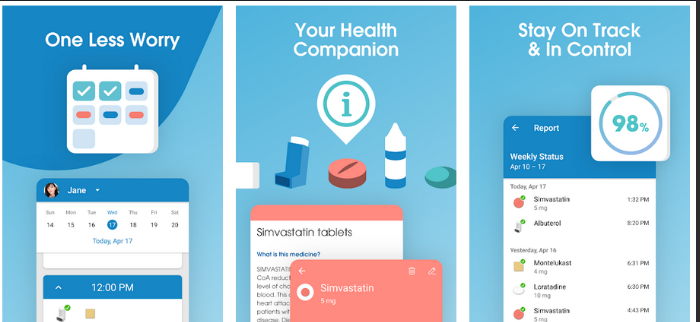
\includegraphics[width=0.7\textwidth]{medisafe.png}
    \caption{Application Medisafe}
    \label{fig:Medisafe}
\end{figure}

\paragraph{Pill Reminder – Meds Alarm :}

\textbf{Avantages :}
\begin{itemize}
    \item Facilité d’utilisation avec une interface intuitive.
    \item Possibilité d’ajouter plusieurs médicaments et d’organiser les prises en fonction des heures de la journée.
\end{itemize}

\textbf{Inconvénients :}
\begin{itemize}
    \item Pas d’interaction avec des proches ou des soignants.
    \item Aucune fonctionnalité de gestion des urgences ni de journal de suivi.
    \item Pas d’intégration avec des assistants vocaux ou des options d’accessibilité avancée.
    \item Interface peu attractive.
\end{itemize}
\begin{figure}[H] 
    \centering
    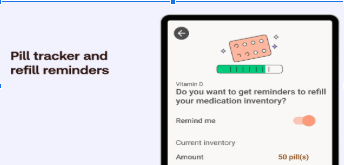
\includegraphics[width=0.7\textwidth]{pill_reminder.png}
    \caption{Application Pill Reminder}
    \label{fig:pillreminder}
\end{figure}
\paragraph{Google Calendar :}

\textbf{Avantages :}
\begin{itemize}
    \item Gratuit et disponible sur tous les appareils.
    \item Permet de planifier des rappels avec répétition automatique.
    \item Partage de calendrier avec les proches.
\end{itemize}

\textbf{Inconvénients :}
\begin{itemize}
    \item Non spécifiquement conçu pour les personnes âgées.
    \item Pas de fonctionnalités de gestion des médicaments ou d’urgence.
    \item Dépendance à un compte Google.
\end{itemize}
\begin{figure}[H] 
    \centering
    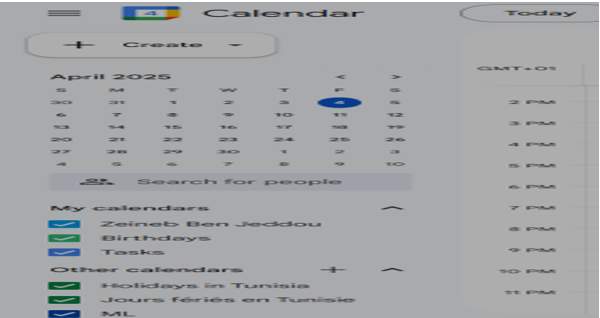
\includegraphics[width=0.7\textwidth]{googleCalender.png}
    \caption{Application Google Calender}
    \label{fig:googleCalender}
\end{figure}
\section{Solution proposée}

L’analyse des solutions existantes a mis en évidence plusieurs limites qui empêchent une gestion efficace des rappels médicaux et des interactions entre les personnes âgées, leurs proches et les soignants.

Pour pallier ces insuffisances, nous proposons de développer une application mobile intelligente d’assistance aux personnes âgées, intégrant des fonctionnalités adaptées à leurs besoins spécifiques.

\textbf{Fonctionnalités proposées :}
\begin{itemize}
    \item \textbf{Gestion des rappels} : prise de médicaments et rendez-vous médicaux.
    \item \textbf{Interaction} : partage de calendrier, notifications, et messagerie.
    \item \textbf{Accessibilité} : interface intuitive avec boutons larges, polices lisibles, et assistance vocale.
    \item \textbf{Chatbot intelligent} : pour aider à programmer les rappels et répondre aux questions.
    \item \textbf{Journal de suivi} : historique des rappels et interactions.
    \item \textbf{Bouton SOS} : envoi d’une alerte géolocalisée aux proches en cas d’urgence.
\end{itemize}

Toutes ces fonctionnalités sont intégrées dans un système sécurisé, performant et évolutif.

\section{Choix méthodologiques}

\subsection{Formalisme de modélisation}

Pour la spécification des besoins, nous avons opté pour le langage de modélisation UML, qui permet la description et la visualisation des exigences ainsi que la définition de l’architecture logicielle.

Nous avons utilisé :
\begin{itemize}
    \item \textbf{Diagramme de cas d’utilisation} : pour visualiser le comportement global de l’application.
    \item \textbf{Diagramme de classes} : pour définir la structure de l’application.
    \item \textbf{Diagramme de séquences} : pour décrire les interactions entre les éléments du système et les acteurs.
\end{itemize}

\subsection{Méthodologie Scrum}

Depuis plusieurs années, les méthodes agiles, et en particulier Scrum, ont été adoptées pour assurer une gestion réactive et itérative des projets.

\paragraph{Présentation de la méthode Scrum :}

Scrum est une méthode agile créée en 2002. Le nom vient du rugby, où la “mêlée” représente l’organisation collective autour d’un objectif. Les projets Scrum sont découpés en itérations courtes appelées \textbf{Sprints} (1 à 3 semaines), permettant une évaluation et planification régulières.

\paragraph{Principaux éléments :}

\begin{itemize}
    \item \textbf{Product Backlog} : Liste des besoins fonctionnels (sous forme de User Stories).
    \item \textbf{User Story} : Description littérale et non technique d’une fonctionnalité.
    \item \textbf{Sprint Backlog} : Liste des User Stories à développer pendant un Sprint.
    \item \textbf{Sprint} : Itération courte ayant un objectif précis.
    \item \textbf{Task} : Une User Story est décomposée en tâches élémentaires.
\end{itemize}

\paragraph{Répartition des rôles :}

\begin{itemize}
    \item \textbf{Product Owner} : Représente le client final, priorise les besoins.
    \item \textbf{Scrum Master} : Facilite le processus Scrum, lève les obstacles.
    \item \textbf{Équipe de développement} : Auto-organisée, multidisciplinaire, réalise les tâches.
\end{itemize}

\paragraph{Processus Scrum :}
\begin{figure}[H] 
    \centering
    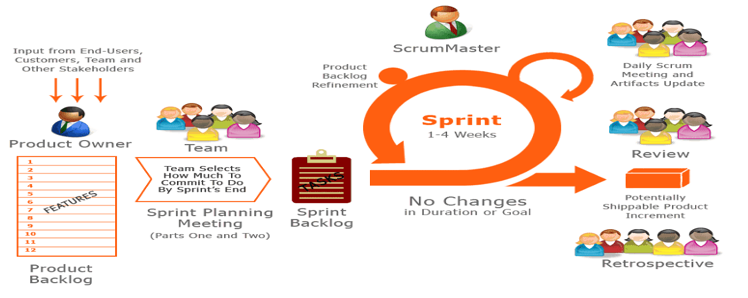
\includegraphics[width=0.7\textwidth]{processusScrum.png}
    \caption{Processus Scrum}
    \label{fig:processusScrum}
\end{figure}
Chaque Sprint commence par une réunion de planification pour fixer les objectifs, puis s’exécute avec une revue de Sprint et une rétrospective. Un diagramme illustre généralement ce cycle complet.
\section{Conclusion}
Dans ce chapitre, nous avons effectué une étude critique de l’existant en présentant notre solution qui va remédier aux insuffisances de l’application actuelle. Nous avons terminé le chapitre en introduisant la méthodologie ainsi que le formalisme de modélisation que nous avons adopté pour la conception du projet que nous allons spécifier dans le chapitre suivant.
\chapter{Sprint Zéro}

\section{Introduction}

Dans ce chapitre intitulé \textbf{Sprint Zéro}, nous présentons les premières étapes préparatoires du projet. Le Sprint Zéro (ou Sprint 0) ne se termine pas forcément par une livraison, mais permet de définir les bases du projet : exigences, participants, backlog initial, etc.

\section{Spécification des besoins}

\subsection{Identification des acteurs}

Un acteur est une entité externe interagissant avec le système. Dans notre application, les principaux acteurs sont :

\begin{longtable}{|p{4cm}|p{5cm}|p{6cm}|}
\hline
\textbf{Acteur} & \textbf{Description} & \textbf{Actions principales} \\
\hline
Utilisateur (personne âgée / proche) & Utilisateur principal de l’application. Bénéficie de l’assistance pour les rappels, la communication et la sécurité. & 
\begin{itemize}
    \item Recevoir des rappels.
    \item Gérer les tâches quotidiennes.
    \item Contacter les proches ou soignants.
    \item Activer le bouton SOS.
\end{itemize} \\
\hline
Soignant & Professionnel de santé assurant le suivi. & 
\begin{itemize}
    \item Accéder aux rappels.
    \item Consulter le journal de suivi.
    \item Être alerté en cas d’urgence.
\end{itemize} \\
\hline
\caption{Tableau d'acteurs }
    \label{tab:tabActeur}
\end{longtable}

\subsection{Spécifications des besoins fonctionnels}

\paragraph{Pour la personne âgée :}
\begin{itemize}
    \item Être assistée via rappels et notifications.
    \item Pouvoir communiquer avec proches et soignants.
    \item Utiliser un chatbot pour poser des questions.
    \item Suivre ses traitements et rendez-vous.
    \item Améliorer son autonomie.
\end{itemize}

\paragraph{Pour l’aidant :}
\begin{itemize}
    \item Recevoir des alertes de suivi.
    \item Accéder aux données de santé.
    \item Aider la personne âgée sans intrusion.
\end{itemize}

\subsection{Spécifications des besoins non fonctionnels}

\begin{itemize}
    \item \textbf{Extensibilité} : ajout futur de nouvelles fonctionnalités.
    \item \textbf{Sécurité} : confidentialité et authentification sécurisée.
    \item \textbf{Interface graphique} : lisibilité et ergonomie pour utilisateurs seniors.
    \item \textbf{Maintenance} : code source clair et documenté.
    \item \textbf{Performance} : réactivité et temps de réponse rapides.
\end{itemize}

\section{Pattern et style architectural}

\subsection{Style architectural – Architecture trois-tiers}

L’architecture trois-tiers (\textit{three-tier architecture}) permet une séparation logique des rôles dans l’application :

\begin{itemize}
    \item \textbf{Client} : Interface utilisateur (mobile Flutter) ;
    \item \textbf{Serveur d'application (middleware)} : Spring Boot, qui traite les requêtes et applique la logique métier ;
    \item \textbf{Serveur de base de données} : MySQL, pour stocker les données des utilisateurs, rappels, profils, etc.
\end{itemize}

Cette séparation permet une meilleure performance, sécurité et évolutivité.

\subsection{Pattern architectural – MVC}

Le modèle MVC (Modèle-Vue-Contrôleur) structure l’application en trois composants :
\begin{figure}[H] 
    \centering
    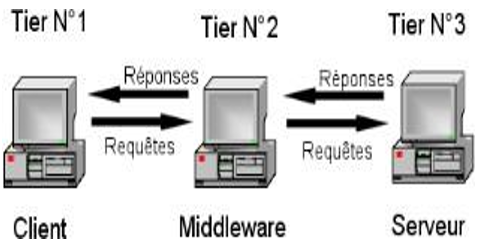
\includegraphics[width=0.7\textwidth]{modele.png}
    \caption{modèle MVC}
    \label{fig:modeleMVC}
\end{figure}
\begin{itemize}
    \item \textbf{Modèle} : Contient la logique métier et gère les données (ex. : objets Utilisateur, Médicament).
    \item \textbf{Vue} : Interface utilisateur, affichant les informations (UI Flutter).
    \item \textbf{Contrôleur} : Traite les entrées utilisateurs, appelle les modèles et met à jour la vue.
\end{itemize}

Ce découpage rend le développement modulaire et facilite la maintenance.
\begin{figure}[H] 
    \centering
    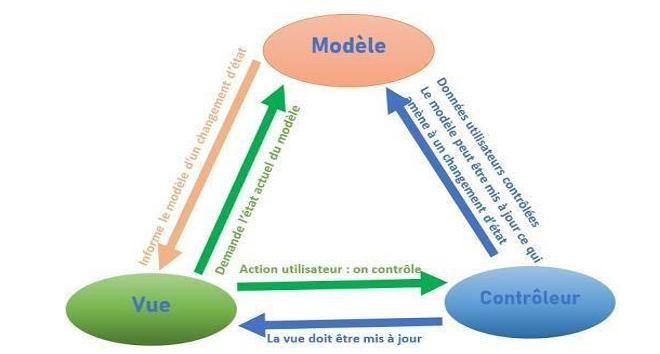
\includegraphics[width=0.7\textwidth]{archi.png}
    \caption{architecture MVC}
    \label{fig:archiMVC}
\end{figure}
\subsection{Pattern architectural – MVVM}

MVVM (Model-View-ViewModel) est une variante moderne du MVC adaptée aux frameworks comme Flutter :

\begin{itemize}
    \item \textbf{Model} : Gestion des données comme dans MVC.
    \item \textbf{View} : Affichage, sans logique métier.
    \item \textbf{ViewModel} : Lien entre vue et modèle, gère les données observables et la logique d’interface.
\end{itemize}

Ce modèle est adapté aux architectures réactives et à l’usage des états dans Flutter.
\begin{figure}[H] 
    \centering
    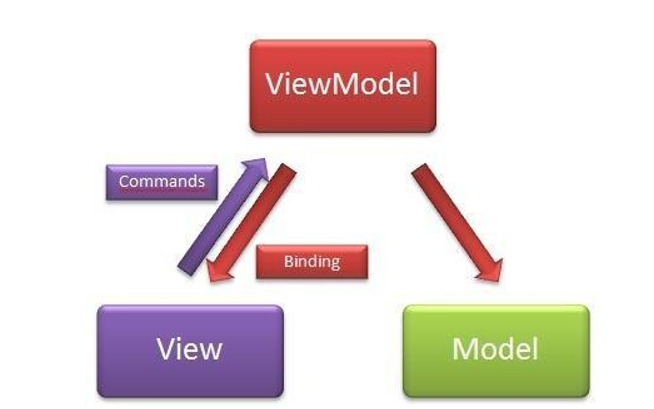
\includegraphics[width=0.7\textwidth]{archi2.png}
    \caption{architecture MVVM}
    \label{fig:archiMVVM}
\end{figure}
\section{Planning du traitement des cas d’utilisation}

\subsection{Importance et exigences}

Certaines fonctionnalités sont plus prioritaires que d’autres. Pour cela, une planification par niveau d’importance est utilisée : élevé, moyen, faible.

Cette hiérarchisation permet de développer d’abord les fonctionnalités critiques et dépendantes des autres.

\subsection{Backlog produit}
\item ID : Identifiant unique de la fonctionnalité.
\item Fonctionnalité : Désignation de la fonctionnalité à implémenter.
\item User Story : Description du besoin utilisateur formulé 
\item Priorité : Niveau d’importance de la user story
\begin{longtable}{|p{1.5cm}|p{4cm}|p{1.5cm}|p{7cm}|p{1.5cm}|}
\hline
\textbf{ID} & \textbf{Fonctionnalité} & \textbf{ID Story} & \textbf{User Story} & \textbf{Priorité} \\
\hline
1 & Authentification & 1.1 &- En tant qu’utilisateur, je peux m’authentifier pour accéder à l’application. & Élevée \\
\hline
2 & Gestion utilisateurs & 2.1 &- En tant que personne âgée, je peux mettre à jour mes informations personnelles. & Élevée \\
& & 2.2 &- En tant qu’aidant, je peux consulter la liste des personnes âgées sous ma responsabilité. & Moyenne \\
& & 2.3 &- En tant qu’aidant, je peux afficher des infos par utilisateur & Moyenne \\
\hline
3 & Aide et assistance & 3.1 &- En tant que personne âgée, je peux envoyer une demande d’aide à un aidant. & Élevée \\
& & 3.2 &- En tant qu’aidant, je peux voir et répondre aux demandes d’aide & Élevée \\
& & 3.3 &- En tant qu’aidant, je peux suivre l’état des demandes d’assistance. & Moyenne \\
\hline
4 & Notifications & 4.1 & -	En tant que personne âgée, je peux recevoir des rappels pour mes médicaments. & Élevée \\
& & 4.2 & -	En tant qu’aidant, je peux être notifié lorsqu'une personne âgée demande de l’aide. & Élevée \\
\hline
5 & Messagerie & 5.1 & -	En tant que personne âgée, je peux envoyer des messages à mon aidant. & Moyenne \\
& & 5.2 & -	En tant qu’aidant, je peux envoyer des messages aux personnes âgées dont je m’occupe. & Moyenne \\
\hline
6 & Suivi de santé & 6.1 & -	En tant que personne âgée, je peux enregistrer mes données de santé (tension, glycémie…). & Faible \\
& & 6.2 & -	En tant qu’aidant, je peux consulter l’historique des données de santé d’une personne âgée. & Moyenne \\
\hline
\caption{Backlog global }
\label{backlog}
\end{longtable}

\subsection{Structure et découpage du projet – Sprints}
\item Sprint : Itération de développement Agile.
\item Description du contenu : Fonctionnalités à réaliser durant le sprint.
\item Durée : Temps alloué en jours pour le sprint.
\begin{longtable}{|p{2.5cm}|p{9cm}|p{3cm}|}
\hline
\textbf{Sprint} & \textbf{Description du contenu} & \textbf{Durée} \\
\hline
Sprint 1 & Authentification + Mise à jour des infos + Consultation des profils & 10 jours \\
\hline
Sprint 2 & Envoi/réception des demandes d’aide + Notifications médicales + Alertes d’urgence & 15 jours \\
\hline
Sprint 3 & Fonctionnalité de messagerie & 4 jours \\
\hline
Sprint 4 & Enregistrement et historique des données santé & 7 jours \\
\hline
\caption{Décomposition des sprints }
\label{sprints}
\end{longtable}
\section{Technologies et outils de développement}

\subsection{Développement back-end}

\paragraph{Spring Boot :}

Spring Boot est un framework Java qui facilite la création d'applications autonomes et prêtes à l'emploi. Il permet une configuration simplifiée et une gestion efficace des services backend.
\begin{figure}[H] 
    \centering
    
\includegraphics[width=0.2\textwidth]{spring-boot.png}
    \caption{Spring Boot}
    \label{fig:springboot}
\end{figure}

\paragraph{MySQL :}

MySQL est un système de gestion de base de données relationnelle (SGBDR) open-source. Il est performant, évolutif et compatible avec SQL. Il permet de stocker les données liées aux utilisateurs, rappels, messages, etc.
\begin{figure}[H] 
    \centering
    
\includegraphics[width=0.2\textwidth]{Mysql.png}
    \caption{MySQL}
    \label{fig:mysql}
\end{figure}

\paragraph{Chatbot Gemini :}

Gemini est un modèle avancé d'intelligence artificielle développé par Google. Il permet d’intégrer un chatbot intelligent pour assister l’utilisateur : rappels, navigation, questions fréquentes, etc.
\begin{figure}[H] 
    \centering
    
\includegraphics[width=0.2\textwidth]{gemini.jpeg}
    \caption{Gemini}
    \label{fig:gemini}
\end{figure}
\subsection{Développement front-end}

\paragraph{Flutter :}

Flutter est un framework UI open-source développé par Google. Il permet de créer des applications mobiles multiplateformes (Android et iOS) avec un seul code source en Dart.
\begin{figure}[H] 
    \centering
    
\includegraphics[width=0.2\textwidth]{flutter.png}
    \caption{Flutter}
    \label{fig:flutter}
\end{figure}

Ses avantages incluent :
\begin{itemize}
    \item Développement rapide avec hot reload.
    \item Interface fluide et moderne.
    \item Intégration facile avec des APIs (Firebase, REST, etc.)
\end{itemize}
\subsection{ Environnement de développement}

\subsubsection*{Matériel utilisé}
\begin{figure}[H] 
    \centering
    
\includegraphics[width=0.2\textwidth]{pc.jpeg}
    \caption{ Matériel utilisé}
    \label{fig:pc}
\end{figure}
\begin{itemize}
    \item \textbf{Modèle} : ASUS TUF Gaming F15 (FX507VV-LP287W)
    \item \textbf{Processeur} : Intel Core i7-13620H (10 cœurs, jusqu’à 4.9 GHz)
    \item \textbf{Mémoire vive} : 16 Go DDR5 4800 MHz 
    \item \textbf{Stockage} : SSD NVMe PCIe 4.0 de 512 Go
    \item \textbf{Carte graphique} : NVIDIA GeForce RTX 4060 8 Go GDDR6 (TGP jusqu’à 140W)
    \item \textbf{Écran} : 15,6'' FHD (1920 x 1080), IPS, 144 Hz, 250 nits
    \item \textbf{Système d’exploitation} : Windows 11 
\end{itemize}

\vspace{0.3cm}

\subsubsection*{Outils et environnements logiciels}
\begin{itemize}
    \item \textbf{IDE Back-end} : IntelliJ IDEA
    \begin{figure}[H] 
    \centering
    
\includegraphics[width=0.2\textwidth]{intellij.jpeg}
    \caption{IntelliJ IDEA }
    \label{fig:intellij}
\end{figure}
    \item \textbf{IDE Front-end} : Visual Studio Code
    \begin{figure}[H] 
    \centering
    
\includegraphics[width=0.2\textwidth]{vscode.jpeg}
    \caption{Visual Studio Code}
    \label{fig:vscode}
\end{figure}
    \item \textbf{SDK Flutter} : Flutter SDK 3.x
      \begin{figure}[H] 
    \centering
    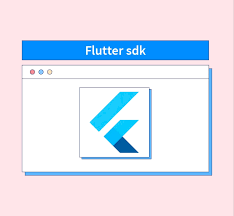
\includegraphics[width=0.2\textwidth]{sdk.png}
    \caption{Flutter SDK 3.x}
    \label{fig:sdk}
\end{figure}
    \item \textbf{JDK} : OpenJDK 17
         \begin{figure}[H] 
    \centering
    
\includegraphics[width=0.2\textwidth]{jdk.png}
    \caption{OpenJDK 17}
    \label{fig:jdk}
\end{figure}
    \item \textbf{Base de données} : MySQL Server 8.x
             \begin{figure}[H] 
    \centering
    
\includegraphics[width=0.2\textwidth]{sq.png}
    \caption{MySQL Server 8.x}
    \label{fig:sq}
\end{figure}
    \item \textbf{Outils de test} : Postman (pour les API REST)
                 \begin{figure}[H] 
    \centering
    
\includegraphics[width=0.2\textwidth]{postman.png}
    \caption{Postman }
    \label{fig:postman}
\end{figure}
    Android Studio (pour l’émulation Android)
                     \begin{figure}[H] 
    \centering
    
\includegraphics[width=0.2\textwidth]{as.png}
    \caption{Android Studio }
    \label{fig:AS}
\end{figure}
\end{itemize}

\section{Modélisation UML}

La modélisation UML permet de visualiser le comportement et la structure du système à travers des diagrammes standardisés.

\subsection{Diagramme de cas d’utilisation}

Ce diagramme montre les interactions entre les différents acteurs (personne âgée, aidant) et les fonctionnalités du système.

\begin{itemize}
    \item Authentification
    \item Modification des informations
    \item Consultation des informations
    \item Envoi de demandes d’aide
    \item Réponse aux alertes
    \item Consultation de l’historique
\end{itemize}
 
\begin{figure}[H] 
    \centering
    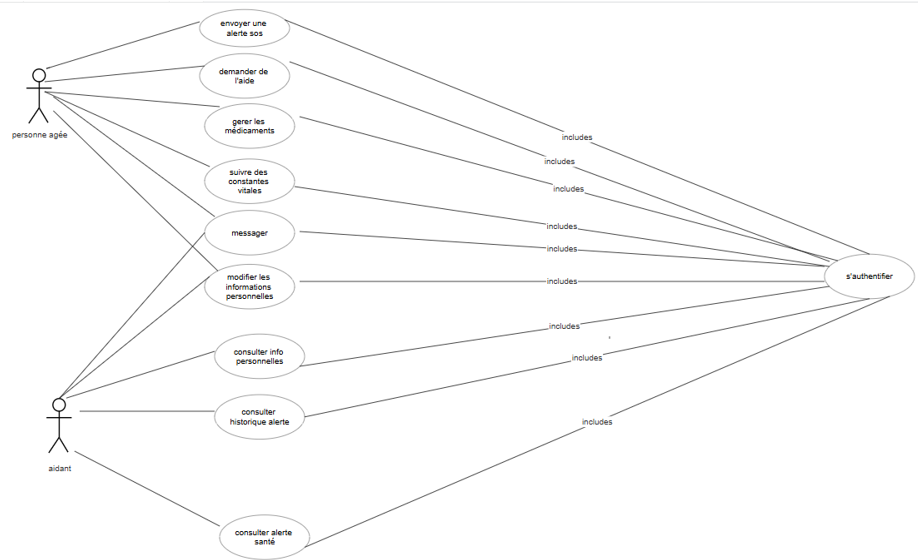
\includegraphics[width=0.7\textwidth]{cas_utilisation.png}
    \caption{Diagramme des cas d'utilisation}
    \label{fig:uses_case}
\end{figure}


\subsection{Diagramme de classes}

Ce diagramme représente les entités principales de l'application et leurs relations.

\begin{itemize}
    \item Utilisateur (Personne âgée, Aidant)
    \item DemandeAide
    \item Notification
    \item Rappel
    \item Message
    \item SuiviSanté
\end{itemize}
 
\begin{figure}[H] 
    \centering
    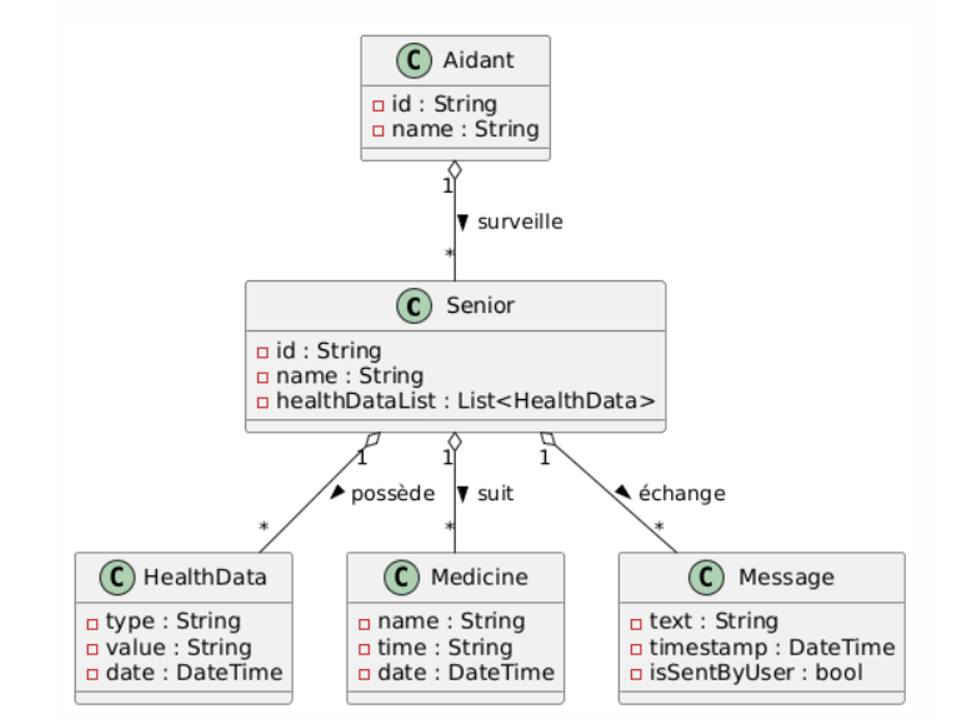
\includegraphics[width=0.7\textwidth]{diagramme_classes.png}
    \caption{Diagramme de classes }
    \label{fig:classe}
\end{figure}


\subsection{Diagramme de séquences}

Ce diagramme illustre les échanges entre les composants lors d’un scénario précis (ex : authentification ou alerte SOS).
 
\begin{figure}[H] 
    \centering
    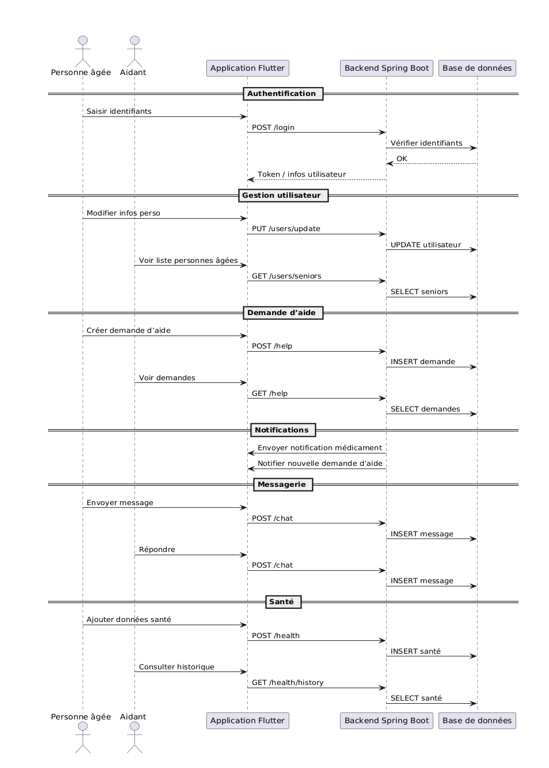
\includegraphics[width=0.7\textwidth]{sequence.png}
    \caption{Diagramme de séquences}
    \label{fig:sequence}
\end{figure}
\section{Conclusion}
Dans ce chapitre, nous avons planifié notre travail en suivant les instructions de l'approche de conception Scrum. Ainsi, nous avons défini les spécifications et les exigences de l’application à développer. Après, nous avons publié le backlog du produit contenant une liste des fonctionnalités attendues de l’application et nous avons cité quelques prototypes d’interfaces. De plus, nous avons préparé la répartition du sprint . Dans le chapitre suivant, nous allons commencer à modéliser le projet en commençant par le premier sprint. 
\chapter{Sprint 1}

\section{Introduction}

Dans le chapitre précédent, nous avons défini la spécification des exigences. Ensuite, nous avons divisé le projet en sprints. Chaque sprint spécifie une période durant laquelle le développement doit être fait et revu. Dans ce sens, nous détaillons dans ce chapitre le premier sprint qui comprend  l’authentification de l’utilisateur, la mise à jour des informations personnelles, ainsi que la consultation de la liste des informations personnelles par l’aidant.
\section{Backlog du sprint}
\item ID : Identifiant de la User Story
\item User Story : Besoins exprimés par l’utilisateur.
\item Tâche : Actions nécessaires pour réaliser la User Story 

\begin{longtable}{|p{2cm}|p{5cm}|p{7cm}|}
\hline
\textbf{ID} & \textbf{User Story} & \textbf{Tache} \\
\hline
1.1 & En tant qu’utilisateur, je peux m’authentifier.& -Réaliser les diagrammes des cas d’utilisation, de séquence et de classes : « S’authentifier »

-Développer le cas « S’authentifier » (Frontend + Backend)

-Tester le cas « S’authentifier » (tests fonctionnels + unitaires)
 \\
\hline
2.1 & En tant que personne âgée, je peux mettre à jour mes informations personnelles. & -Réaliser les diagrammes des cas d’utilisation, de séquence et de classes : « Modifier profil »

-Développer la fonctionnalité « Modifier profil » (modification nom, âge, santé...)

-Tester la mise à jour des informations personnelles
 \\
\hline
2.2 & En tant qu’aidant, je peux consulter la liste des personnes âgées sous ma responsabilité. &- Réaliser les diagrammes des cas d’utilisation, de séquence et de classes : « Consultation utilisateurs »

-Développer la consultation des profils des personnes âgées par l’aidant

-Tester la consultation des informations côté aidant
 \\
\hline
\caption{Backlog du sprint 1}
\label{backlogSprint1}
\end{longtable}

\section{Spécifications fonctionnelles}

\subsection{Classification des cas d’utilisation par acteur }
\textbf{Personne agée :} 
S’authentifier , Modifier ses informations personnelles , Consulter ses informations personnelles  
\\
\textbf{Aidant :} S’authentifier , Modifier ses informations personnelles , Consulter ses informations personnelles 
 \\
 \subsection{Diagramme de cas d'utilisation de sprint 1}
\begin{figure}[H] 
    \centering
    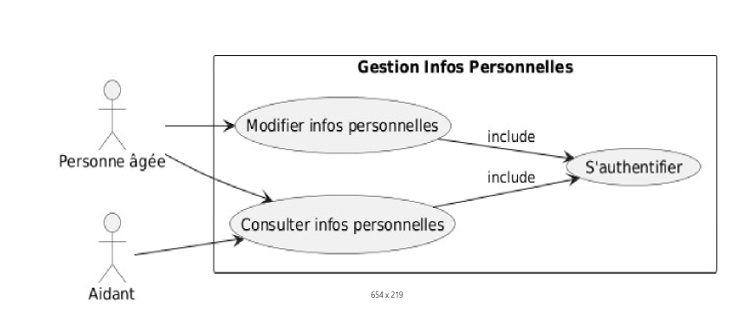
\includegraphics[width=0.7\textwidth]{sprint1.png}
    \caption{Diagramme de  cas d'utilisation de sprint 1}
    \label{fig:diagSprint1}
\end{figure}
-	La personne âgée peut réaliser l’ensemble des cas d’utilisation relatifs à la gestion de son compte. Elle peut ainsi s’authentifier, modifier ses informations personnelles, et consulter ses informations personnelles.

-	L’aidant dispose des mêmes fonctionnalités. Il peut également s’authentifier, modifier ses informations personnelles et consulter les informations personnelles de la personne aidée.

-	Chaque action inclut obligatoirement une phase d’authentification préalable, représentée par une relation <<include>> dans le diagramme.

\subsection{Cas d’utilisation : S’authentifier}
\begin{figure}[H] 
    \centering
    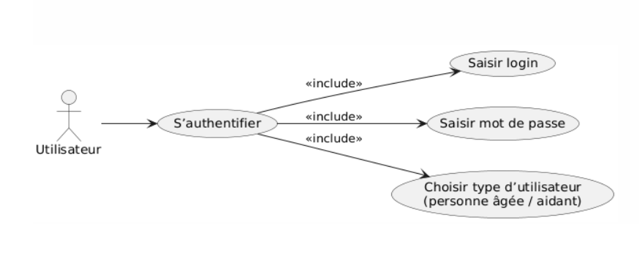
\includegraphics[width=0.7\textwidth]{s'authentifier.png}
    \caption{cas d'utilisation : s'authentifier}
    \label{fig:s'authentifier}
\end{figure}
\textbf{Acteurs :} Personne âgée, Aidant \\
\textbf{Préconditions :} L’utilisateur est enregistré dans le système. \\
\textbf{Postcondition :} Accès à l’espace personnel (aidant ou senior).

\paragraph{Scénario principal :}
\begin{enumerate}
    \item L’utilisateur lance l’application.
    \item Il saisit son adresse e-mail et mot de passe.
    \item Il choisit son rôle (senior ou aidant).
    \item Il clique sur “Se connecter”.
    \item Le système valide et redirige vers la page d’accueil.
\end{enumerate}

\paragraph{Scénario alternatif :}
\begin{itemize}
    \item Email ou mot de passe incorrect → message d’erreur.
    \item Champ vide → affichage d’un message de validation.
\end{itemize}

\subsection{Cas d’utilisation : Modifier les informations personnelles}
\begin{figure}[H] 
    \centering
    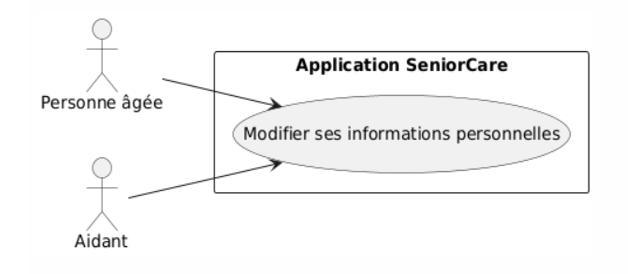
\includegraphics[width=0.7\textwidth]{modifier.png}
    \caption{Cas d'utiliation : Modifier les informations personnelles }
    \label{fig:modifierSprint1}
\end{figure}
\textbf{Acteurs :} Utilisateur authentifié \\
\textbf{Préconditions :} Accès à la section “Mon Profil”. \\
\textbf{Postcondition :} Les nouvelles informations sont sauvegardées.

\paragraph{Scénario principal :}
\begin{enumerate}
    \item Accès à “Mon Profil”.
    \item Clic sur “Modifier”.
    \item Saisie des nouvelles informations.
    \item Validation.
    \item Mise à jour dans la base + message de confirmation.
\end{enumerate}

\paragraph{Scénario alternatif :}
\begin{itemize}
    \item Champ vide ou invalide → message d’erreur, annulation de la mise à jour.
\end{itemize}

\subsection{Cas d’utilisation : Consulter les informations personnelles}
\begin{figure}[H] 
    \centering
    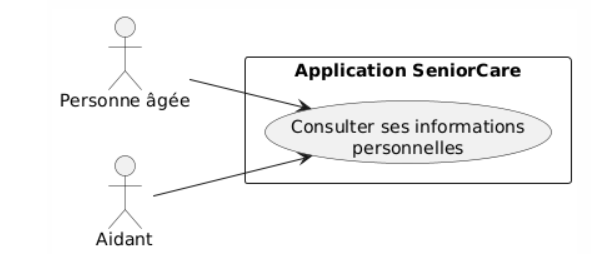
\includegraphics[width=0.7\textwidth]{consulter.png}
    \caption{Cas d'utilisation : Consulter les informations personnelles }
    \label{fig:consulterSprint1}
\end{figure}
\textbf{Acteurs :} Utilisateur connecté \\
\textbf{Préconditions :} Authentification réussie \\
\textbf{Postcondition :} Affichage des données

\paragraph{Scénario principal :}
\begin{enumerate}
    \item Clic sur l’icône “Mon Profil”
    \item Chargement des données
    \item Affichage sur écran
\end{enumerate}

\paragraph{Scénario alternatif :}
\begin{itemize}
    \item Erreur de chargement → affichage d’un message d’erreur
\end{itemize}
\section{Interfaces utilisateur}

\subsection{Écran d’authentification}

Cet écran permet à l’utilisateur (personne âgée ou aidant) de saisir ses identifiants pour accéder à son espace personnel.

\begin{itemize}
    \item Champs : nom d'utilisateur, Mot de passe
    \item Bouton : Se connecter
    \item Options : Mot de passe oublié, Créer un compte
\end{itemize}
 
\begin{figure}[H] 
    \centering
    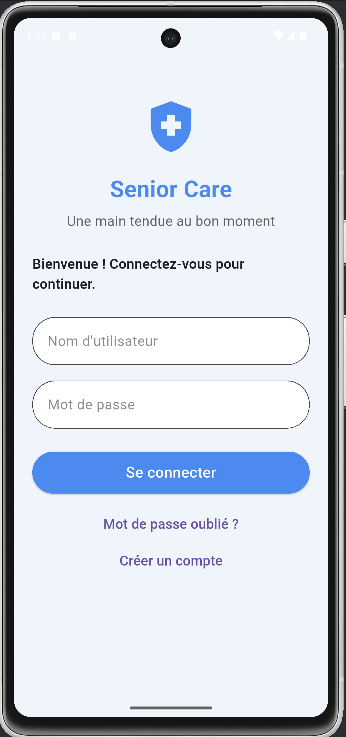
\includegraphics[width=0.5\textwidth]{login_screen1.png}
    \caption{Ecran d'authentification }
    \label{fig:ecranAuthentification}
\end{figure}
\subsection{Écran de création de compte}

\begin{itemize}
    \item Saisie : Nom,  Mot de passe
    \item Sélection du rôle (senior ou aidant)
    \item Bouton : Créer un compte
\end{itemize}

\begin{figure}[H] 
    \centering
    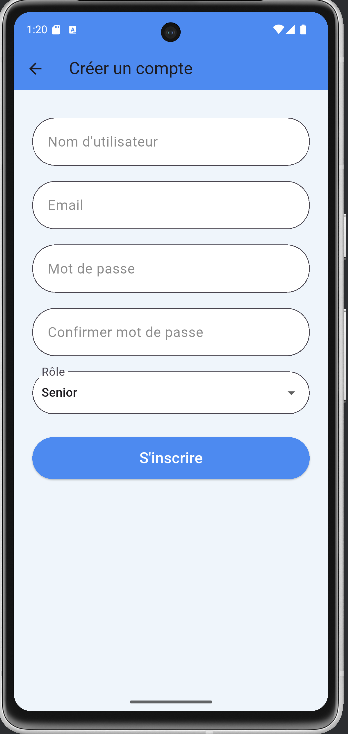
\includegraphics[width=0.5\textwidth]{register_screen1.png}
    \caption{Ecran de création de compte  }
    \label{fig:ecranCreation}
\end{figure}
\subsection{Écran du mot de passe oublié}
\begin{itemize}
    \item Saisie : Email
    \item Bouton : Envoyer
\end{itemize}
\begin{figure}[H] 
    \centering
    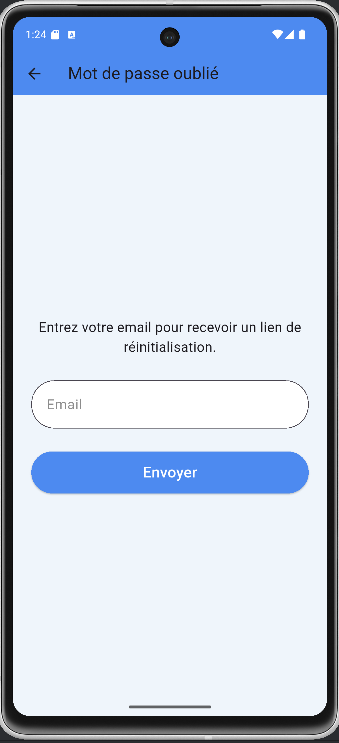
\includegraphics[width=0.5\textwidth]{password_screen1.png}
    \caption{Ecran du mot de passe oublié }
    \label{fig:ecranPassword}
\end{figure}
\subsection{Tableau de bord Aidant}
\begin{figure}[H] 
    \centering
    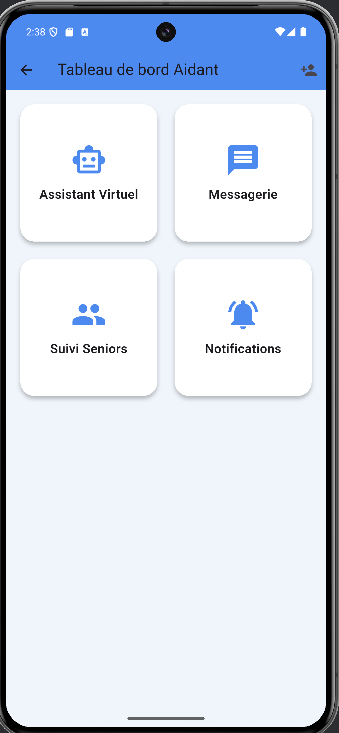
\includegraphics[width=0.5\textwidth]{aidant.png}
    \caption{Tableau de bord Aidant  }
    \label{fig:aidant}
\end{figure}
\subsection{Tableau de bord Senior”}
\begin{figure}[H] 
    \centering
    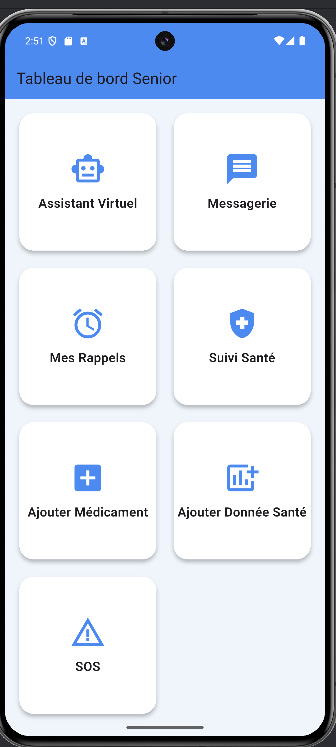
\includegraphics[width=0.5\textwidth]{senior.png}
    \caption{Tableau de bord Senior }
    \label{fig:senior}
\end{figure}
\section{Conclusion}
Dans la première phase du projet, nous avons réussi à vérifier le premier sprint. Maintenant, nous avons le premier incrément de l'application. Dans le prochain chapitre, nous allons concevoir et développer un deuxième Sprint 

\end{document}